\documentclass[11pt]{article}

% ACL style (review mode for anonymous ARR submission)
\usepackage[review]{acl}

% Standard packages from official ACL template
\usepackage{times}
\usepackage{latexsym}
\usepackage[T1]{fontenc}
\usepackage[utf8]{inputenc}
\usepackage{microtype}
\usepackage{inconsolata}

% Math
\usepackage{amsmath}
\usepackage{amssymb}

% Tables
\usepackage{booktabs}
\usepackage{multirow}
\usepackage{tabularx}

% Graphics (xcolor loaded by acl.sty)
\usepackage{graphicx}
\graphicspath{{../../artifacts/}}

% Lists
\usepackage{enumitem}

% Custom commands
\newcommand{\cls}{\textsc{Cls}}
\newcommand{\cwm}{\textsc{Cwm}}
\newcommand{\traj}{\textsc{Traj}}
\newcommand{\fone}{F\textsubscript{1}}
\newcommand{\pp}{\,\text{pp}}

\title{A Systematic Comparison of Execution-Free Verification Formulations for Code Repair}
\author{Anonymous}

\begin{document}
\maketitle

\begin{abstract}
LLM-based program repair increasingly relies on generating multiple candidate patches and selecting the best via a verifier. Execution-based verification is reliable but expensive; three execution-free alternatives have emerged: per-test binary classification (\cls{}), execution output generation (\cwm{}), and trajectory-level patch scoring (\traj{}). No prior work compares these formulations under matched conditions.

We present the first systematic comparison across two representative code LLM families (Qwen3, DeepSeek-Coder), two complexity levels, and multiple seeds under ${\leq}$8B LoRA fine-tuning. Our primary finding is function-level near-equivalence: \cls{} and \cwm{} achieve statistical equivalence across both families (TOST $p{=}0.007$, $\pm$2\pp{} margin, 5 seeds, Holm-Bonferroni corrected), establishing that classification is not inherently easier than generation when outputs are short (${\leq}$1.3\pp{} gap). \traj{} reaches parity on Qwen3 but exceeds the equivalence margin on DeepSeek-Coder (2.69\pp{}), revealing model-dependent sensitivity. At repository level, a robust per-test interaction ($z{=}-23.7$, $n{=}56{,}480$) confirms this equivalence breaks: the \cls{}--\cwm{} gap widens from ${\leq}$1.3\pp{} to 19--26\pp{} in single-seed variant-level evaluation, driven by format collapse in generation-based simulation; gap magnitude depends on multiple confounds.

Error complementarity across formulations (oracle ensemble: 90.63\%) and a failure mode taxonomy motivate complexity-aware formulation routing over uniform selection.
\end{abstract}

\section{Introduction}
\label{sec:introduction}

LLM-based automated program repair systems increasingly rely on test-time compute scaling: generating $K$ candidate patches and selecting the best via a verifier~\cite{snell2024scaling}. Full execution verification is reliable but expensive (\$1--3 per candidate at repository scale\footnote{Based on per-instance costs reported by \citet{yang2024sweagent} and \citet{xia2024agentless}.}), driving demand for execution-free alternatives. Three distinct formulations have emerged for this task: \textbf{generation-based simulation}~\cite{meta2025cwm,maimon2026selfexecution} predicts execution output strings per test; \textbf{trajectory-level scoring}~\cite{shum2025swerm} predicts a binary patch verdict without per-test decomposition; and \textbf{per-test classification}~\cite{ni2023lever,chen2023codet} predicts a pass/fail token per test. Each makes different tradeoffs between diagnostic granularity, output complexity, and inference cost.

Despite active development along each axis, no prior work provides a controlled comparison holding model capacity, training data, and compute constant. Practitioners choosing a formulation for their verification pipeline must rely on results from different models, different datasets, and different evaluation protocols. Whether one formulation is uniformly preferable, or whether the choice depends on properties of the code being verified, remains an open empirical question. A related question is whether formulation choice matters at all relative to more basic decisions: at what complexity level does fine-tuning become necessary, and does formulation selection add value beyond what fine-tuning alone provides?

We present the first systematic comparison of these three formulations across two model families (Qwen3, DeepSeek-Coder), two complexity levels (function-level and repository-level), and multiple seeds. Our results reveal a three-layer structure in the verification design space. Repository-level verification is inherently harder than function-level (0-shot accuracy drops below majority baseline). Fine-tuning is necessary under standard prompting (0-shot$\to$fine-tuned gains of 25--35\pp{} at repo level). Even after fine-tuning, \emph{formulation choice is governed by a formulation $\times$ model $\times$ complexity interaction}: at function-level complexity, all three formulations achieve statistically equivalent accuracy; at repository-level complexity, formulations diverge sharply, with the divergence being formulation-inherent in direction but model-contingent in magnitude. Figure~\ref{fig:reformulation} illustrates the three formulations.

We make the following contributions:

\begin{itemize}[leftmargin=*,itemsep=2pt]
\item \textbf{Formulation equivalence at low complexity.} On function-level benchmarks, \cls{}, \cwm{}, and \traj{} achieve near-identical accuracy across two model families (Qwen3-4B: 88.4/87.2/86.3\%, 5 seeds; DeepSeek-6.7B: 86.9/86.8\%, 2 seeds). The \cls{}--\cwm{} gap is 0.02--1.24\pp{}, within seed noise in both cases. This null result establishes that classification is not inherently easier than generation when execution outputs are short and structured.

\item \textbf{Complexity-dependent divergence with formulation $\times$ model interaction.} At repository-level complexity, \cls{} achieves 19--26\pp{} higher accuracy than \cwm{} on Qwen3. Cross-model validation with DeepSeek-Coder confirms the divergence is formulation-inherent: both families show \cwm{} $\gg$ \cls{} degradation from function to repo level (Qwen3: ${\sim}$5/22\pp{}; DeepSeek: ${\sim}$12/25\pp{} for \cls{}/\cwm{}). The magnitude is model-contingent: DeepSeek exhibits larger \cls{} degradation (${\sim}$12\pp{} vs.\ ${\sim}$5\pp{}). %%SCENARIO-A%% Beyond accuracy, \cwm{} exhibits higher seed sensitivity at repo level (${\sim}$5\pp{} across seeds vs.\ ${\sim}$2\pp{} for \cls{}), while showing no overtraining under our protocol. %%END-SCENARIO-A%%

\item \textbf{Error complementarity and ensemble potential.} \cls{} and \cwm{} exhibit systematically opposite error patterns at function level: \cls{} over-predicts passing (75.5\% of errors are false negatives) while \cwm{} over-predicts failure (83.1\% false positives). An oracle ensemble achieves 90.63\% (+3.12\pp{} over the best single formulation). The formulations appear to capture complementary aspects of code behavior.

\item \textbf{Diagnostic granularity at equivalent accuracy.} Per-test classification achieves statistically equivalent variant-level accuracy to trajectory-level scoring (TOST equivalence $p = 0.007$, $\pm$2\pp{} margin) while providing per-test diagnostic information at 217$\times$ higher throughput than generation (1 output token vs.\ avg 477). Whether this additional granularity translates to downstream improvements (e.g., targeted re-repair) remains an open question.
\end{itemize}


\begin{figure*}[t]
\centering
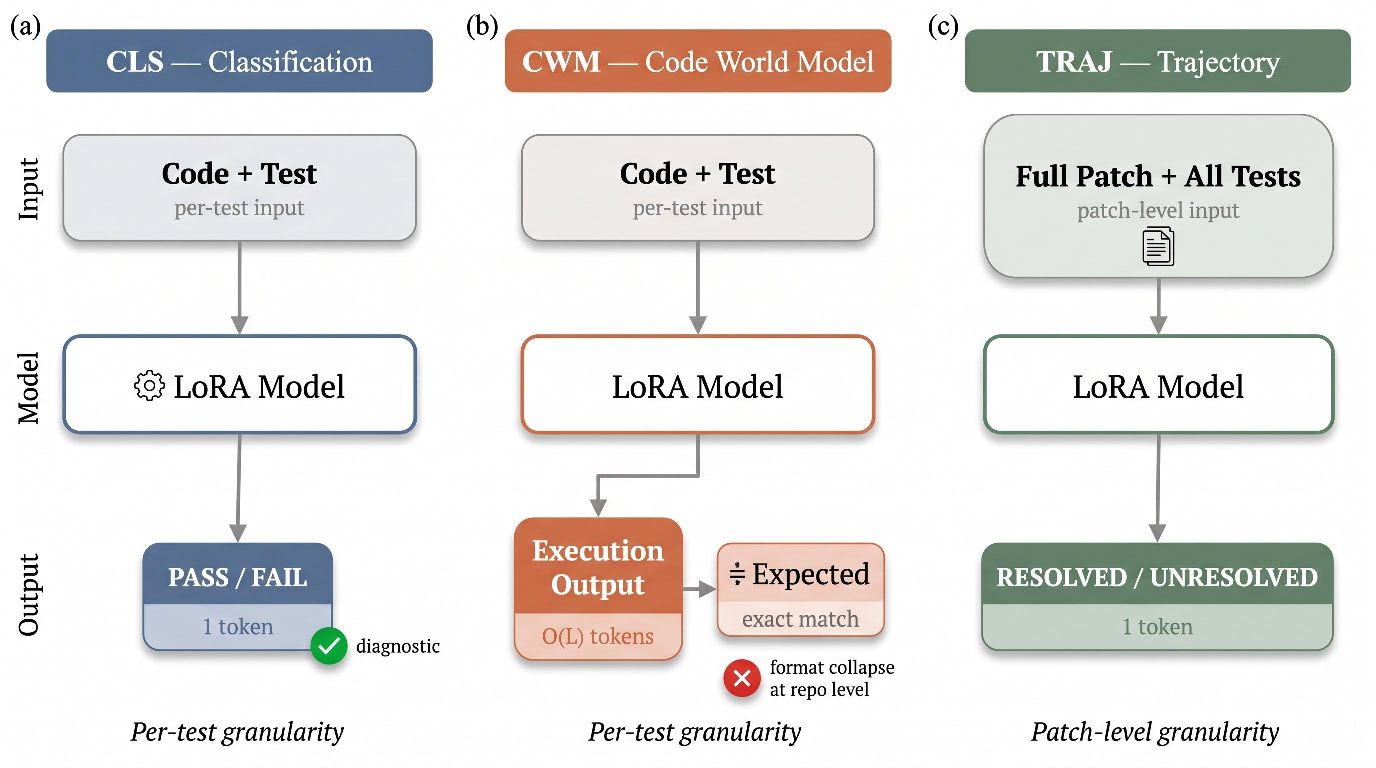
\includegraphics[width=\textwidth]{figures/paper/fig1_reformulation.pdf}
\caption{Three verification formulations. \textbf{Left:} \cls{} predicts binary pass/fail per test (1 output token). \textbf{Center:} \cwm{} generates execution output, derives verdict by exact match ($O(L)$ tokens). \textbf{Right:} Trajectory-level scoring predicts patch-level resolved/unresolved (1 token, no per-test signal). Each formulation makes different tradeoffs between output complexity, diagnostic granularity, and inference cost.}
\label{fig:reformulation}
\end{figure*}

\section{Related Work}
\label{sec:related_work}

\paragraph{Code World Models and Execution Simulation.}
Code World Models~\cite{meta2025cwm} mid-train a 32B LLM on execution traces to predict output strings and establish the generation-based paradigm for execution-free verification.
Self-Execution~\cite{maimon2026selfexecution} extends this with step-by-step trace prediction.
CodeMind~\cite{liu2024codemind} evaluates code reasoning along multiple dimensions including execution prediction.
SolidCoder~\cite{lee2026solidcoder} bridges mental simulation and actual execution via concrete feedback.
Abdollahi et al.~\cite{abdollahi2025demystifying} identify systematic failure modes in LLM trace prediction, including position-dependent errors.
All share a generation formulation whose cost scales with output length. We provide the first controlled comparison of this formulation against classification and trajectory-level alternatives at matched model capacity.

\paragraph{Execution-free Verification.}
SWE-RM~\cite{shum2025swerm} trains a trajectory-level reward model for patch ranking without execution.
Patch Reasoner~\cite{xu2025patchreasoner} uses chain-of-thought reasoning for patch verification.
LEVER~\cite{ni2023lever} trains a classifier to re-rank code candidates by predicting execution correctness; CodeT~\cite{chen2023codet} uses dual execution agreement as a verification signal.
ICE-Score~\cite{zhuo2024icescore}, CodeScore~\cite{dong2024codescore}, and CodeBERTScore~\cite{zhou2023codebertscore} evaluate code quality without execution via learned metrics, but target generation quality assessment rather than per-test pass/fail verification.
Snell et al.~\cite{snell2024scaling} show that test-time scaling via verification outperforms parameter scaling; S*~\cite{li2025sstar} and VG-Search~\cite{chen2025vgsearch} find that finer-grained verification improves selection efficiency.
Self-consistency~\cite{wang2023selfconsistency} uses majority voting over sampled solutions as an implicit verifier.
These works treat verification granularity and formulation as design choices but do not compare them at controlled capacity. We isolate the formulation variable (classification vs.\ generation vs.\ trajectory-level) while holding model, data, and compute constant.

\paragraph{Process vs.\ Outcome Supervision.}
Lightman et al.~\cite{lightman2023letsverify} demonstrate that process-based reward models (verifying each reasoning step) outperform outcome-based models (verifying only the final answer) for mathematical reasoning.
Uesato et al.~\cite{uesato2022solving} show similar advantages for process feedback in math word problems.
In code, DreamPRM-Code~\cite{dreamprm2025code} applies function-level process rewards, and PRL-Coder~\cite{ye2025prlcoder} integrates process supervision into RL-based code generation.
Our per-test classification is structurally analogous to process supervision: each test verdict corresponds to an intermediate verification step, while trajectory-level scoring corresponds to outcome supervision. Our finding that per-test and trajectory-level achieve equivalent accuracy (TOST $p = 0.007$) with per-test providing additional diagnostic value parallels the process supervision result that step-level verification enables error localization at no accuracy cost.

\paragraph{Verification in Repair Pipelines.}
CodeRL~\cite{le2022coderl} trains a critic model to provide execution feedback for RL-based code generation.
AlphaCode~\cite{li2022alphacode} and AlphaCode 2~\cite{alphacode2023team} use massive sampling with test-based filtering for competition programming.
Reflexion~\cite{shinn2023reflexion} uses verbal self-reflection on execution results to iteratively improve agent performance.
SWE-bench~\cite{jimenez2024swebench} and SWE-bench Verified~\cite{chowdhury2024swebenchverified} provide standard benchmarks; SWE-agent~\cite{yang2024sweagent} and Agentless~\cite{xia2024agentless} demonstrate agent-based and pipeline-based repair respectively.
Yang et al.~\cite{yang2025aprsurvey} survey LLM-based repair, identifying verification as a persistent bottleneck with cost scaling linearly in candidates.
These systems demonstrate that verification quality is a primary bottleneck for iterative repair. Our formulation comparison is complementary: the efficiency and diagnostic granularity of the verifier directly affects the viability of verification-in-the-loop approaches at scale.

\paragraph{Predictive Mutation Testing.}
Predicting test outcomes for code mutations without execution has been studied in software engineering~\cite{tufano2019predictive,kim2022predictive}, with recent work applying LLMs to mutation testing~\cite{wang2024llmmutation} and contextual prediction~\cite{jain2023contextual}. Our per-test classification shares this problem structure: given a code change and a test, predict pass or fail. We extend this line to LLM-based verification at repository scale, comparing it against generation and trajectory-level formulations under controlled conditions for the first time.

\paragraph{Parameter-Efficient Fine-Tuning for Code.}
LoRA~\cite{hu2022lora} enables low-rank adaptation of large models with minimal trainable parameters; QLoRA~\cite{dettmers2024qlora} extends this to quantized models.
Both have become standard for code-specific fine-tuning, with DeepSeek-Coder~\cite{guo2024deepseekcoder} demonstrating that adapter-based training preserves pretrained code understanding while specializing for downstream tasks.
We use LoRA (rank 16) for all experiments to ensure that capacity differences between formulations reflect the task structure rather than total trainable parameters. Our rank ablation (Appendix~\ref{app:ablations}) confirms that doubling adapter capacity does not resolve the generation bottleneck, consistent with a formulation-level constraint rather than a capacity limitation.

\paragraph{Classification vs.\ Generation in NLP.}
Task framing affects model performance broadly: T5~\cite{raffel2020t5} and BART~\cite{lewis2020bart} demonstrate generation-classification tradeoffs under controlled capacity, while SQuAD~\cite{rajpurkar2016squad} shows that constraining output space can simplify tasks without sacrificing quality. We extend this lens to code verification, finding that code complexity moderates the tradeoff in a model-contingent manner.


\section{Method}
\label{sec:method}

Let $p$ denote a candidate patch and $T = \{t_1, \ldots, t_n\}$ its test suite, where each $t_i$ has label $y_i \in \{\text{\textsc{Pass}}, \text{\textsc{Fail}}\}$ from execution. Tests decompose into \emph{fail-to-pass} ($T_{\text{f2p}}$) and \emph{pass-to-pass} ($T_{\text{p2p}}$) subsets; a patch is correct iff $\forall\, t_i{:}\ y_i = \text{\textsc{Pass}}$. We compare three formulations for predicting correctness without execution.

\subsection{Verification Formulations}
\label{sec:formulations}

Let $c_p$ denote the code context (unified diff) of patch $p$.

\paragraph{\cls{} (per-test classification).} $f(c_p, t_i) \rightarrow \hat{y}_i \in \{\text{\textsc{Pass}}, \text{\textsc{Fail}}\}$ predicts a single binary token per test (cross-entropy loss). Patch verdict: $\hat{y}_p = \bigwedge_{i} [\hat{y}_i = \text{\textsc{Pass}}]$. Output cost: one token per test.

\paragraph{\cwm{} (output generation).} $g(c_p, t_i) \rightarrow \hat{o}_i \in \Sigma^*$ generates the execution output string (language modeling loss). Verdict by exact match: $\hat{y}_i = \text{\textsc{Pass}}$ iff $\hat{o}_i = o_i^*$.\footnote{Exact string matching is conservative, consistent with \citet{meta2025cwm}. Semantic equivalences are not counted.} When the generated output is unparseable (i.e., does not conform to the expected structured format), the prediction defaults to the majority class verdict. Output cost: $\sum_i |\hat{o}_i|$ tokens.

\paragraph{\traj{} (trajectory-level).} $h(c_p, T) \rightarrow \hat{y}_p \in \{\text{\textsc{Resolved}}, \text{\textsc{Unresolved}}\}$ predicts a single patch verdict from all tests, providing no per-test signal. \traj{} serves as a granularity control: \cls{}--\traj{} differences isolate the value of per-test decomposition independent of the classification formulation itself.

\subsection{Formulation-Specific Failure Modes}
\label{sec:failure-modes}

Each formulation has characteristic failure modes that differ in their sensitivity to code complexity:

\paragraph{Generation failure modes (\cwm{}).} The open-ended output space introduces three failure modes: (1)~\emph{token-budget exhaustion}, where $|o_i^*| > B$ guarantees exact-match failure due to truncation; (2)~\emph{string-value prediction errors}, where semantically equivalent outputs differing in surface form (floating-point precision, dictionary ordering) produce false negatives; and (3)~\emph{format compliance collapse}, where the model fails to produce structured predictions entirely at high input complexity, even when the generation budget is sufficient. Under optimistic independence, a token sequence of length $L$ with per-token accuracy $q$ has correct-sequence probability $q^L$, making long outputs exponentially harder to predict exactly. We adopt exact string matching following the original \cwm{} evaluation protocol~\citep{meta2025cwm}. Unparseable predictions default to the majority-class label (\textsc{Pass}).

\paragraph{Classification failure modes (\cls{}).} The single-token output space eliminates format and truncation failures but constrains the model to encode its reasoning entirely within internal representations, without the intermediate reasoning trace that generation provides. \cls{} errors concentrate in false negatives (predicting \textsc{Pass} for failing tests), consistent with a bias toward the majority class.

\paragraph{Trajectory-level failure modes (\traj{}).} By collapsing all per-test information into a single binary verdict, \traj{} discards diagnostic granularity. When a patch fails multiple tests, the trajectory-level formulation cannot identify \emph{which} tests fail. This limits downstream utility (e.g., targeted re-repair) but avoids per-test aggregation errors.

\paragraph{Complexity dependence.} These failure modes suggest a complexity-dependent interaction: when execution outputs are short and structured (function-level code), generation modes (1)--(2) are rarely triggered, and all formulations should perform comparably. As output length and structural complexity increase (repository-level code), generation-specific failures may compound, creating divergence. Whether this divergence reflects a fundamental property of the generation formulation or is contingent on model/tokenizer properties is an empirical question we investigate in \S\ref{sec:experiments}.

\subsection{Oracle Accuracy-Utility Framework}
\label{sec:oracle}

Per-test granularity is valuable only when per-test predictions are sufficiently accurate and multiple tests provide partially independent signals. Consider a buggy patch with $k = |T_{\text{f2p}}|$ fail-to-pass tests. A per-test verifier with recall $r$ detects the bug if it identifies at least one failing test:
%
\begin{equation}
  P_{\text{detect}}(k) = 1 - (1 - r)^{k_{\text{eff}}}
  \label{eq:pdetect}
\end{equation}
%
where $k_{\text{eff}}$ is the effective number of independent tests. Let $a_h$ denote the trajectory-level detection accuracy; it is independent of $k$.

\paragraph{Block-correlation model.} Per-test predictions within the same patch are correlated. We model this via the intraclass correlation coefficient $\rho$ \citep[ICC;][]{shrout1979icc}:
%
\begin{equation}
  k_{\text{eff}} = \frac{k}{1 + (k - 1)\rho}
  \label{eq:keff}
\end{equation}
%
When $\rho = 0$, $k_{\text{eff}} = k$ (full independence); when $\rho = 1$, $k_{\text{eff}} = 1$ (per-test collapses to trajectory-level). The per-test advantage relative to a trajectory-level baseline is $\Delta(k) = P_{\text{detect}}(k) - a_h$, and the expected population advantage is:
%
\begin{equation}
  \mathbb{E}[\Delta] = \sum_{k=1}^{K} P(|T_{\text{f2p}}| = k) \cdot \Delta(k)
  \label{eq:expected-advantage}
\end{equation}

\paragraph{Testable predictions.} This yields three predictions validated in \S\ref{sec:experiments}: (1)~at $k = 1$, $\Delta \approx 0$; (2)~$\Delta(k)$ increases with $k$, dampened by $\rho > 0$; (3)~$\mathbb{E}[\Delta]$ concentrates in multi-F2P-test instances.


\section{Experiments}
\label{sec:experiments}

We evaluate \cls{}, \cwm{}, and trajectory-level scoring (TRAJ) across model sizes and complexity levels.

\subsection{Experimental Setup}
\label{sec:setup}

\paragraph{Datasets.}
\emph{Function-level}: mutated variants from HumanEval~\cite{chen2021humaneval} and MBPP~\cite{austin2021mbpp} (five mutation types), labels verified by execution. 19,076 samples (train 15,290 / val 1,896 / test 1,890; pass:fail $\approx$ 52:48, majority baseline 51.75\%).
\emph{Repo-level}: per-test instances from SWE-bench Verified~\cite{chowdhury2024swebenchverified} mutants. ${\sim}$70K training samples; val ($n{=}9{,}335$) and test ($n{=}9{,}784$) have zero problem overlap (majority baseline 72.96\%). Val-based checkpoint selection follows standard practice~\cite{jimenez2024swebench}.

\paragraph{Models and training.}
We fine-tune Qwen3-4B and Qwen3-8B~\cite{qwen2025qwen3} with LoRA~\cite{hu2022lora} (rank 16, 3 epochs) across five seeds. Seeds 42/123/456 use bfloat16; seeds 789/0 use NF4 quantization~\cite{dettmers2024qlora}. Our \cwm{} baseline is a LoRA fine-tuned variant for controlled comparison, not a reproduction of the 32B Code World Model~\cite{meta2025cwm}. Repo-level models use val-selected checkpoints. Zero-shot baselines use Qwen3-8B and Qwen3-32B (NF4) as LLM-as-judge.

\paragraph{Statistics.}
Confidence intervals use clustered bootstrap~\cite{davison1997bootstrap} (114 problem clusters, 10K resamples); per-test vs.\ trajectory-level comparison uses TOST~\cite{schuirmann1987tost} ($\pm$2\pp{} margin). ICC~\cite{shrout1979icc} quantifies within-problem correlation. Oracle analysis uses SWE-bench Verified (500 instances).


\subsection{Function-Level Results}
\label{sec:func_results}

Table~\ref{tab:main_results} reports function-level results across formulations.

\begin{table}[t]
\centering
\small
\caption{Function-level per-test verification results on HumanEval+MBPP test set (1,890 samples). \cls{}: per-test binary classification; \cwm{}: execution output generation; TRAJ: trajectory-level scoring; ZS: zero-shot LLM-as-judge. Mean $\pm$ std over seeds reported where applicable.}
\label{tab:main_results}
\resizebox{\columnwidth}{!}{%
\setlength{\tabcolsep}{4pt}
\begin{tabular}{llcc}
\toprule
\textbf{Method} & \textbf{Model} & \textbf{Seeds} & \textbf{Accuracy (\%)} \\
\midrule
\cls{} (fine-tuned) & 4B & 5 & \textbf{88.43 $\pm$ 0.78} \\
\cwm{} (fine-tuned) & 4B & 5 & 87.19 $\pm$ 0.37 \\
TRAJ (fine-tuned) & 4B & 5 & 86.30 $\pm$ 0.97 \\
\midrule
ZS LLM-as-judge & 8B & 1 & 64.40 \\
ZS LLM-as-judge & 32B (NF4) & 1 & 71.69 \\
\bottomrule
\end{tabular}}
\end{table}

Fine-tuned \cls{} achieves 88.43\% ($\pm$0.78), compared to 87.19\% ($\pm$0.37) for \cwm{} and 86.30\% ($\pm$0.97) for TRAJ. The \cls{}--\cwm{} gap is 1.24\pp{}, modest at this complexity level where generation is not yet bottlenecked by token budget or string complexity. Zero-shot baselines lag substantially (64.40\% at 8B, 71.69\% at 32B NF4), confirming that task-specific fine-tuning is necessary for reliable verification.


\subsection{Scaling Behavior}
\label{sec:scaling}

Table~\ref{tab:scaling} compares \cls{} and \cwm{} at two model sizes using three matched seeds (42, 123, 456), all trained in full bfloat16 precision to ensure a controlled comparison.

\begin{table}[t]
\centering
\small
\caption{Model-size scaling: \cls{} vs.\ \cwm{} accuracy (\%) at 4B and 8B. Three matched seeds in full precision. The \cls{}--\cwm{} gap widens from 1.18\pp{} to 2.43\pp{}.}
\label{tab:scaling}
\setlength{\tabcolsep}{4pt}
\begin{tabular}{llccccc}
\toprule
\textbf{Method} & \textbf{Size} & \textbf{s42} & \textbf{s123} & \textbf{s456} & \textbf{Mean} & \textbf{Gap} \\
\midrule
\cls{} & 4B & 87.83 & 89.52 & 87.88 & 88.41 & \multirow{2}{*}{1.18} \\
\cwm{} & 4B & 87.51 & 87.20 & 86.98 & 87.23 & \\
\midrule
\cls{} & 8B & \textbf{90.48} & 89.40 & 88.31 & \textbf{89.40} & \multirow{2}{*}{\textbf{2.43}} \\
\cwm{} & 8B & 87.67 & 86.98 & 86.24 & 86.96 & \\
\bottomrule
\end{tabular}
\end{table}

At 4B, \cls{} and \cwm{} are separated by 1.18\pp{} on the matched three-seed subset. At 8B, the gap more than doubles to 2.43\pp{} (Figure~\ref{fig:scaling_gap}). Clustered bootstrap analysis yields a mean gap of 2.26\pp{} ($p = 0.0066$, 95\% CI $[1.80, 2.71]$), confirming the widening is not a sampling artifact.

The asymmetry in scaling efficiency is striking: from 4B to 8B, \cls{} gains +0.99\pp{} (88.41 $\to$ 89.40) while \cwm{} loses $-$0.27\pp{} (87.23 $\to$ 86.96). The additional model capacity benefits classification---where the model needs only to discriminate pass from fail---but provides no measurable improvement for generation, where the model must additionally produce exact output strings. This pattern is consistent with the hypothesis that the string-prediction bottleneck, not model capacity, bounds \cwm{} accuracy. However, the \cwm{} regression ($-$0.27\pp{}) falls within seed noise (3-seed std ${\sim}$0.5\pp{}) and could reflect suboptimal hyperparameter transfer rather than a fundamental bottleneck. Whether this divergence amplifies at repository-level complexity is examined in \S\ref{sec:repo}.


\subsection{Per-Test vs.\ Trajectory-Level Equivalence}
\label{sec:equivalence}

We compare \cls{} (aggregated via all-pass rule) against TRAJ on 523 variant-level instances across five seeds. The pooled gap is $-$0.45\pp{} (95\% CI [$-$1.71, +0.84]); the TOST equivalence test confirms statistical equivalence at $p = 0.007$ ($\pm$2\pp{} margin). Within-problem predictions are correlated (ICC $= 0.191$, $p < 0.0001$, DEFF $= 3.97$); all statistical tests use clustered bootstrap accordingly. Per-test classification thus provides diagnostic information---which specific tests fail---at no cost to variant-level accuracy.


\subsection{Accuracy-Utility Frontier}
\label{sec:oracle-results}

Oracle analysis on SWE-bench Verified (500 instances) reveals that per-test advantage concentrates sharply: at $T = 1$ F2P tests (68.7\% of instances), per-test and trajectory-level are informationally equivalent. The advantage materializes at $T \geq 2$ (31.3\%), with $T = 2$ alone contributing 55.3\% of the total 10.93\pp{} block-correlated advantage. Full stratification and the i.i.d.\ vs.\ block-correlated comparison appear in Appendix~\ref{app:oracle}.


\subsection{Repo-Level Results}
\label{sec:repo}

Table~\ref{tab:repo_level} compares \cls{} and \cwm{} on SWE-bench Verified per-test classification at repository-level complexity. All checkpoints are selected by validation accuracy; the test set ($n{=}9{,}784$) has zero problem overlap with validation.

\begin{table}[t]
\centering
\small
\caption{Repo-level per-test verification on SWE-bench Verified test set ($n{=}9{,}784$, val-selected checkpoints). Same-size 4B comparison is primary; \cls{} 8B included for scaling context; \cwm{} 8B in progress.}
\label{tab:repo_level}
\resizebox{\columnwidth}{!}{%
\setlength{\tabcolsep}{3pt}
\begin{tabular}{llccccc}
\toprule
\textbf{Method} & \textbf{Size} & \textbf{Seed} & \textbf{Acc (\%)} & \textbf{Macro \fone{}} & \textbf{Unparse (\%)} & \textbf{vs Maj.\ (\pp{})} \\
\midrule
\cls{} & 4B & 42 & \textbf{83.63} & 75.63 & 0.0 & +10.67 \\
\cwm{} & 4B & 42 & 58.04 & 51.67 & 53.7 & $-$14.92 \\
\cwm{} & 4B & 123 & 59.09 & 43.43 & 67.2 & $-$13.87 \\
\midrule
\cls{} & 8B & 42 & 84.48 & 78.17 & 0.0 & +11.52 \\
\cls{} & 8B & 123 & 85.60 & 78.38 & 0.0 & +12.64 \\
\cwm{} & 8B & --- & --- & --- & --- & --- \\
\midrule
Majority & --- & --- & 72.96 & --- & --- & --- \\
\bottomrule
\end{tabular}}
\end{table}

The same-size 4B comparison reveals a 25.59\pp{} gap (\cls{} 83.63\% vs.\ \cwm{} 58.04\%, seed 42; Figure~\ref{fig:scaling_gap}). \cwm{} falls 14.92\pp{} below the majority baseline (72.96\%), indicating negative utility. A second \cwm{} seed (123, 59.09\%) confirms the failure is not seed-specific. The primary driver is format compliance collapse: 53.7--67.2\% of \cwm{} outputs are unparseable across seeds, while \cls{} produces zero unparseable outputs under standard inference (8,192 tokens). Among parseable \cwm{} outputs, accuracy is 42--43\%---below both majority baseline and chance level (50\%)---indicating anti-informative predictions. \S\ref{sec:analysis} provides detailed error analysis.

\cls{} 8B achieves 84.48\% (seed 42) and 85.60\% (seed 123) in cross-size comparison. The 4B$\to$8B transition within \cls{} (83.63\%$\to$84.48\%, seed 42) is within noise (+0.85\pp{}, single seed). \cwm{} 8B evaluation is in progress.

\paragraph{Sequence length.} A matched-context ablation confirms input context disparity explains $<$3\% of the \cls{}--\cwm{} gap: \cls{} 8B evaluated at \texttt{max\_seq\_length}$=$2,048 yields a matched-context gap of 25.00\pp{}, representing 98\% of the same-size 25.59\pp{} gap (Appendix~\ref{app:ablations}).

\paragraph{Limitations.} The same-size 4B comparison uses a single seed; \cls{} 4B seed 123 (val-best ckpt-800) achieves only 75.33\% test accuracy (+2.4\pp{} above majority baseline), indicating that val-best selection at an early checkpoint (step 800) amplifies the val-test distribution shift observed across all configurations. The validation and test sets have zero problem overlap but differ in mutation type composition, introducing potential distribution shift. All repo-level results use val-selected checkpoints, and checkpoint selection variance could contribute to observed differences. Our training data is synthetically constructed from mutation operators rather than real developer patches; the synthetic-to-real transfer gap remains untested, and classifier behavior on naturally occurring bugs may differ from the controlled mutation patterns studied here.


\subsection{Analysis}
\label{sec:analysis}

\paragraph{(a) Error complementarity.}
\cls{} and \cwm{} make errors in opposite directions at function level. Among \cls{} errors (seed 42), 75.5\% are false negatives (FAIL $\to$ PASS), meaning the classifier tends to over-predict passing. Among \cwm{} errors, 83.1\% are false positives (PASS $\to$ FAIL), reflecting string-matching failures that incorrectly reject correct outputs. An oracle combination that takes the correct answer whenever either model is right achieves 90.63\% accuracy, a 3.12\pp{} improvement over \cls{} alone (87.51\%). This complementarity suggests that ensemble approaches combining classification and generation signals could yield further gains.

\paragraph{(b) CWM error mode breakdown.}
Among unparseable \cwm{} outputs, 76.9\% contain no execution keywords; 22.9\% contain ambiguous co-occurring pass/fail keywords. Format compliance varies sharply across repositories (scikit-learn: near-zero unparseable; sphinx: 100\%), suggesting domain-specific code contexts prevent structured generation.

\paragraph{(c) Relaxed matching does not rescue \cwm{}.}
Relaxed matching (tolerating format deviations, L0--L4) \emph{decreases} \cwm{} accuracy: 58.04\%$\to$56.98\% (seed 42) and 59.09\%$\to$55.91\% (seed 123). Unparseable predictions default to the majority class (pass, 72.96\%), which outperforms the model's own parseable predictions (42--53\%). The \cls{}--\cwm{} gap widens from 26\pp{} to 28\pp{}, ruling out the hypothesis that parsing strictness inflates the observed gap.

\paragraph{(d) Variance compression.}
\cwm{}'s 5-seed standard deviation (0.37\pp{}) is lower than \cls{} (0.78\pp{}) and TRAJ (0.97\pp{}) at function level. This is consistent with the bottleneck hypothesis: if \cwm{} performance is capped by output-format constraints, seed-to-seed variability is compressed relative to formulations whose performance depends more on learned representations.

\paragraph{(e) Per-test precision and recall.}
\cls{} achieves fail \fone{} 87.86\% (precision 82.75\%, recall 93.64\%) at seed 42, with 42.1\% of problems perfectly predicted. Multi-F2P instances (6--10 tests) reach 96.3\% accuracy, corroborating the oracle finding.

\paragraph{(f) Block correlation.}
Within-problem errors are correlated (ICC $= 0.191$, DEFF $= 3.97$, 2.81$\times$ more all-correct problems than i.i.d.\ expectation). All tests use clustered bootstrap accordingly.

\paragraph{(g) LoRA rank and majority voting.}
Doubling adapter capacity (rank 32) does not improve \cwm{} accuracy ($-$0.51\pp{}, within seed variance); majority voting ($K{=}3$) decreases accuracy ($-$0.68\pp{}). Both confirm the bottleneck is formulation-level, not capacity-level (Appendix~\ref{app:ablations}).

\section{Conclusion}
\label{sec:conclusion}

We presented the first systematic comparison of three execution-free verification formulations (\cls{}, \cwm{}, \traj{}). At function level, \cls{} and \cwm{} are statistically equivalent (TOST $p{=}0.007$, 5 seeds); \traj{} reaches parity on Qwen3 but not DeepSeek-Coder (2.69\pp{}). Per-test classification achieves 217$\times$ higher throughput while providing diagnostic signal whose downstream utility remains unconfirmed ($n{=}44$, $p{=}0.42$). Complementary errors (oracle: 90.63\%/95.83\%; single-seed) motivate complexity-aware routing. At repository level under ${\leq}$8B LoRA fine-tuning, a significant interaction ($z{=}-23.7$) confirms divergence (19--26\pp{}, single-seed variant-level), with \cwm{} falling below majority baseline---consistent across families but dependent on multiple confounds (\S\ref{sec:threats}). Variant-level analysis reveals three distinct failure modes (format collapse, decision collapse, aggregation penalty) consistent across model families. At function level, formulation choice is immaterial; at repository level under ${\leq}$8B LoRA, \cls{} is recommended for both accuracy and throughput. Behavior at larger scale remains open~\cite{meta2025cwm}.

\section*{Limitations}

Most repo-level comparisons use limited seeds; the gap (19--26\pp{}) exceeds any single assessed confound (\S\ref{sec:threats}), but correlated confounds mean definitive causal attribution requires multi-seed replication. Our \cwm{} baseline uses ${\leq}$8B LoRA fine-tuning, not the original 32B CWM with execution trace mid-training~\cite{meta2025cwm}; at larger scale, the generation bottleneck may diminish. Training data comprises synthetic mutations~\cite{andrews2005mutation,just2014mutants}; the synthetic-to-real transfer gap for absolute accuracy remains untested, though the coupling effect supports relative ranking validity (Appendix~\ref{app:limitations}). Model coverage is limited to 6--8B code-specialized LLMs; generalization to larger or general-purpose models is untested. All code, data, and model checkpoints will be released upon acceptance.

\bibliography{references}

% ARR checklist is filled in OpenReview submission form, not in PDF
% % ARR Responsible NLP Research Checklist
% Reference: https://aclrollingreview.org/responsibleNLPresearch/

\section*{Responsible NLP Research Checklist}

This paper follows the ARR Responsible NLP Research checklist.

\subsection*{A. For Every Submission}

\paragraph{A1. Did you describe the limitations of your work?}
Yes. Section~\ref{sec:conclusion} (Limitations paragraph) discusses: limited seed coverage for repo-level comparisons, synthetic-to-real transfer gap, lack of downstream re-repair validation, and val-test mutation distribution mismatch. Section~\ref{sec:repo} (Limitations paragraph) discusses val-best checkpoint selection variance and seed coverage.

\paragraph{A2. Did you discuss any potential risks of your work?}
This work compares formulations for execution-free code verification on public benchmarks. The primary application is improving automated program repair pipelines. We identify no significant risks: the methods predict test outcomes rather than generating executable code, the datasets are derived from open-source repositories, and no personally identifiable information is involved. Misuse potential is limited because the verifiers require task-specific fine-tuning on labeled data and do not generalize to arbitrary code generation.

\subsection*{B. Did You Use or Create Scientific Artifacts?}

\paragraph{B1. Did you cite the creators of artifacts you used?}
Yes. All datasets (HumanEval~\cite{chen2021humaneval}, MBPP~\cite{austin2021mbpp}, SWE-bench Verified~\cite{chowdhury2024swebenchverified}), models (Qwen3~\cite{qwen2025qwen3}, DeepSeek-Coder~\cite{guo2024deepseekcoder}), and methods (LoRA~\cite{hu2022lora}, QLoRA~\cite{dettmers2024qlora}) are cited in Sections~\ref{sec:setup} and~\ref{sec:formulations}.

\paragraph{B2. Did you discuss the license or terms for use and/or distribution of any artifacts?}
HumanEval is released under MIT license; MBPP under CC-BY-4.0; SWE-bench Verified under MIT license. Qwen3 models are released under Apache 2.0; DeepSeek-Coder under the DeepSeek License. All uses are consistent with their respective licenses. We do not release new artifacts in this submission.

\paragraph{B3. Did you discuss if your use of existing artifact(s) was consistent with their intended use?}
Yes. All benchmarks are used for their intended purpose of evaluating code understanding and generation capabilities. SWE-bench Verified is used for repository-level evaluation as designed by its creators.

\paragraph{B4. Did you discuss the steps taken to check whether the data contains any information that names or uniquely identifies individual people or offensive content?}
Not applicable. Our datasets consist of code snippets and test cases from open-source repositories. The mutation-based data construction process operates on source code only and does not involve personal data or natural language content that could contain offensive material.

\paragraph{B5. Did you provide documentation of the artifacts?}
Yes. Section~\ref{sec:setup} documents dataset statistics (sizes, splits, label distributions, majority baselines). The mutation-based data construction process is described in Section~\ref{sec:setup}. Appendix~\ref{app:hyperparams} provides full hyperparameter details.

\paragraph{B6. Did you report relevant statistics like the number of examples, details of train/test/dev splits, etc.?}
Yes. Section~\ref{sec:setup}: function-level 19,076 samples (train 15,290 / val 1,896 / test 1,890; pass:fail $\approx$ 52:48); repo-level ${\sim}$70K training, val $n{=}9{,}335$, test $n{=}9{,}784$ (majority baseline 72.96\%).

\subsection*{C. Did You Run Computational Experiments?}

\paragraph{C1. Did you report the number of parameters in the models used, the total computational budget, and computing infrastructure?}
Yes. Models: Qwen3-4B (${\sim}$4B parameters, LoRA rank 16 $\approx$ 4M trainable), Qwen3-8B (${\sim}$8B), DeepSeek-Coder-6.7B (${\sim}$6.7B). Infrastructure: 4$\times$ NVIDIA RTX 5090 GPUs. Total compute: ${\sim}$370 GPU-hours across 223 completed runs (${\sim}$46 configurations including seeds, formulations, model sizes, and ablations). Appendix~\ref{app:hyperparams} provides per-run details.

\paragraph{C2. Did you discuss the experimental setup, including hyperparameter search and best-found hyperparameter values?}
Yes. Section~\ref{sec:setup} reports the training configuration (LoRA rank 16, 3 epochs, 5 seeds with mixed precision). Appendix~\ref{app:hyperparams} provides full hyperparameter values. We use a fixed configuration rather than extensive hyperparameter search; repo-level models use validation accuracy for checkpoint selection.

\paragraph{C3. Did you report descriptive statistics about your results with, e.g., error bars or confidence intervals?}
Yes. All multi-seed results report mean $\pm$ standard deviation. Confidence intervals use clustered bootstrap (114 problem clusters, 10K resamples; Section~\ref{sec:setup}). Equivalence testing uses TOST ($p = 0.007$, $\pm$2\pp{} margin; Section~\ref{sec:equivalence}). ICC quantifies within-problem correlation with design effect reported.

\paragraph{C4. If you used existing packages, did you report the implementation and version numbers?}
Yes. Implementation uses HuggingFace Transformers (${\geq}$4.44), PEFT (${\geq}$0.12), PyTorch (${\geq}$2.0), bitsandbytes (${\geq}$0.43, for NF4 quantization), and Python 3.10. LoRA~\cite{hu2022lora} and QLoRA~\cite{dettmers2024qlora} configurations are detailed in Appendix~\ref{app:hyperparams}. Exact version pinning is provided in the code repository.

\subsection*{D. Did You Use Human Annotators?}

Not applicable. This work uses no human annotators or participants. All labels are derived from automated test execution.

\subsection*{E. AI Assistants}

\paragraph{E1. Did you use AI assistants (e.g., ChatGPT, Copilot) in any part of the paper writing or coding process?}
Yes. AI coding assistants were used during development of training and evaluation scripts. AI writing assistants were used for drafting and editing portions of the manuscript. All scientific claims, experimental design, and analysis were conducted and verified by the authors.


\appendix

\section{Oracle Accuracy-Utility Analysis}
\label{app:oracle}

We stratify SWE-bench Verified instances by F2P test count $T$, comparing per-test vs.\ trajectory-level oracle resolve rates under i.i.d.\ and block-correlated error models (ICC $= 0.191$, from function-level TOST analysis; \S\ref{sec:equivalence}).

\begin{table}[h]
\centering
\small
\caption{Oracle accuracy-utility frontier: per-test advantage stratified by F2P test count ($T$) on SWE-bench Verified (500 instances). Block-correlated model uses function-level ICC $= 0.191$ (from TOST equivalence analysis). P2P regression rate: 1.04\% mean, 0\% median.}
\label{tab:oracle}
\resizebox{\columnwidth}{!}{%
\setlength{\tabcolsep}{3pt}
\begin{tabular}{lcccc}
\toprule
\textbf{$T$} & \textbf{Inst.\%} & \textbf{i.i.d.\ (\pp{})} & \textbf{Block (\pp{})} & \textbf{Contrib.\%} \\
\midrule
$1$ & 68.7 & $-$0.04 & $-$0.09 & $\approx$0 \\
$2$ & 19.1 & 18.49 & 31.69 & 55.3 \\
$3$--$5$ & 7.1 & 25.00 & 40.74 & $\approx$26 \\
$\geq 6$ & 5.1 & 30.00 & 40.06 & $\approx$19 \\
\midrule
\textbf{All} & 100.0 & --- & \textbf{10.93} & 100.0 \\
\bottomrule
\end{tabular}}
\end{table}

\begin{figure}[h]
\centering
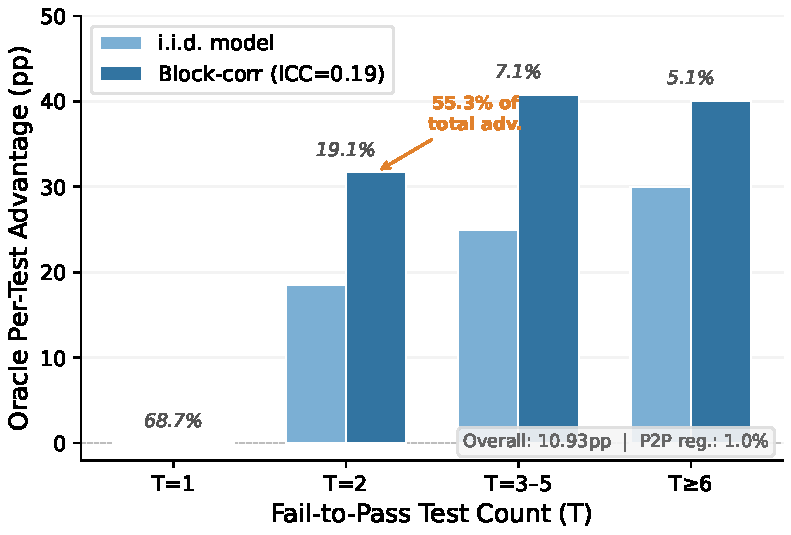
\includegraphics[width=\columnwidth]{figures/paper/fig3_oracle_stratified.pdf}
\caption{Oracle per-test advantage by F2P test count $T$. Advantage is zero at $T{=}1$ (68.7\%) and concentrates at $T{=}2$ (19.1\%, contributing 55.3\% of total advantage).}
\label{fig:oracle_stratified}
\end{figure}

Table~\ref{tab:oracle} and Figure~\ref{fig:oracle_stratified} reveal a sharp concentration: at $T = 1$ (68.7\% of instances), per-test and trajectory-level are informationally equivalent. The advantage materializes at $T = 2$ (19.1\%), where block-correlated advantage reaches 31.69\pp{} (55.3\% of total). The overall block-correlated advantage is 10.93\pp{}, driven by the $T \geq 2$ minority. Block correlation amplifies relative to i.i.d.: at $T = 2$, 31.69\pp{} vs.\ 18.49\pp{} (1.7$\times$). P2P regression is negligible (1.04\% mean, 0\% median); the practical value concentrates in F2P discrimination.

\paragraph{Sensitivity to ICC estimate.}
The analysis above uses ICC $= 0.191$ from function-level TOST equivalence testing (\S\ref{sec:equivalence}), where mean cluster size $\bar{k} \approx 16.5$ yields DEFF $= 3.97$. At repository level, within-problem correlation is substantially stronger: ICC $= 0.3146$ with DEFF $= 114.4$ (\S\ref{sec:repo}), reflecting the larger and more heterogeneous test suites in SWE-bench Verified problems. Under higher ICC, within-problem errors cluster more tightly, amplifying the block-correlated per-test advantage at each $T$ stratum---the correction from i.i.d.\ to block-correlated grows monotonically with ICC. The function-level ICC $= 0.191$ used in Table~\ref{tab:oracle} thus provides a conservative lower bound on the per-test advantage; the repo-level correlation structure would yield an even larger gap between per-test and trajectory-level oracle resolve rates, strengthening the case for per-test granularity at repository-level complexity.

\section{Ablation Studies}
\label{app:ablations}

\paragraph{LoRA rank sensitivity.}
All \cwm{} experiments use LoRA rank $r{=}16$. To test whether this capacity constraint handicaps \cwm{}, we train rank-32 variants (seed 42), doubling adapter parameters.

\begin{table}[h]
\centering
\small
\caption{LoRA rank ablation for \cwm{} 4B (seed 42, 3 epochs, lr $= 2{\times}10^{-4}$). Rank-16 seed variance: 0.53\pp{} (seeds 42 vs.\ 456).}
\label{tab:rank_ablation}
\setlength{\tabcolsep}{4pt}
\begin{tabular}{lccccc}
\toprule
\textbf{Config} & \textbf{$\alpha/r$} & \textbf{Acc (\%)} & \textbf{Fail \fone{}} & \textbf{Pass \fone{}} & \textbf{$\Delta$} \\
\midrule
$r{=}16$, $\alpha{=}32$ & 2 & \textbf{87.51} & --- & --- & --- \\
$r{=}32$, $\alpha{=}32$ & 1 & 87.00 & 87.1 & 86.9 & $-$0.51 \\
$r{=}32$, $\alpha{=}64$ & 2 & 87.04 & 87.27 & 86.79 & $-$0.47 \\
\bottomrule
\end{tabular}
\end{table}

Both rank-32 variants fall within the 2-seed variance of the rank-16 baseline (0.53\pp{} between seeds 42 and 456). The $\alpha{=}64$ variant (matching the baseline $\alpha/r{=}2$ ratio) rules out the confound that the $\alpha{=}32$ result might reflect reduced effective scaling rather than rank insensitivity. This is consistent with \cwm{}'s function-level performance being bounded by output-format constraints rather than adapter capacity.

\paragraph{Majority voting.}
Majority voting ($K{=}3$) decreases accuracy from 87.51\% to 86.83\% ($-$0.68\pp{}): errors are systematic rather than stochastic, so sampling-based ensembles do not help.

\paragraph{Sequence-length ablation details.}
Both formulations are trained with \texttt{max\_seq\_length}$=$2,048. At inference, \cwm{} reserves \texttt{max\_new\_tokens}$=$1,024, leaving ${\sim}$1,024 effective input tokens; \cls{} allocates nearly all context to input (5,120--8,192 tokens). A matched-context ablation (\cls{} 8B at 2,048 tokens) achieves 83.04\%, only 1.44\pp{} below the 8,192-token evaluation (84.48\%), though truncation introduces 136 unparseable outputs (1.39\% of test samples). The matched-context gap (\cls{}@2,048 vs.\ \cwm{}@2,048) is 25.00\pp{}---98\% of the full 25.59\pp{} gap---confirming that input context disparity explains at most 3\% of the difference.

\section{Repo-Level Per-Mutation Breakdown}
\label{app:repo_mutation}

Table~\ref{tab:mutation_breakdown} compares per-mutation accuracy at repo level. \cls{} produces 0\% unparseable outputs; all values are direct classification accuracy. \cwm{} overall accuracy includes default-pass assignment for unparseable outputs (see \S\ref{sec:repo}).

\begin{table}[h]
\centering
\small
\caption{Per-mutation test accuracy (\%) at repo level (SWE-bench Verified, $n{=}9{,}784$). \cls{} 8B reports two seeds; $\Delta$ is mean 4B$\to$8B gain for \cls{}. \cwm{} 4B per-mutation overall accuracy unavailable except gold (computed from parse rate 43.5\%, parseable acc 23.5\%).}
\label{tab:mutation_breakdown}
\resizebox{\columnwidth}{!}{%
\setlength{\tabcolsep}{3pt}
\begin{tabular}{lccccccc}
\toprule
\textbf{Mutation} & \textbf{$n$} & \textbf{CLS 4B} & \textbf{CLS 8B s42} & \textbf{CLS 8B s123} & \textbf{CWM 4B} & \textbf{CWM 8B} & \textbf{$\Delta$ CLS} \\
\midrule
gold & 4,633 & 98.25 & 96.24 & 99.60 & 66.72 & 80.06 & $-$0.33 \\
operator\_swap & 3,357 & 78.91 & 81.38 & 82.60 & --- & 54.57 & +3.08 \\
off\_by\_one & 183 & 58.47 & 86.89 & 79.20 & --- & 63.39 & \textbf{+24.58} \\
return\_value & 562 & 67.97 & 75.44 & 66.40 & --- & 49.11 & +2.95 \\
boundary\_removal & 1,049 & 46.90 & 46.90 & 44.90 & --- & 42.23 & $-$1.00 \\
\bottomrule
\end{tabular}}
\end{table}

Table~\ref{tab:cwm_mutation_parse} shows that \cwm{} generation quality degrades from 4B to 8B across all mutation types.

\begin{table}[h]
\centering
\small
\caption{\cwm{} parse rates and parseable-only accuracy per mutation type (seed 42). Parse rate decreases uniformly from 4B to 8B; parseable-only accuracy is below random binary chance (50\%) for gold at both scales.}
\label{tab:cwm_mutation_parse}
\setlength{\tabcolsep}{4pt}
\begin{tabular}{lcccc}
\toprule
& \multicolumn{2}{c}{\textbf{Parse Rate (\%)}} & \multicolumn{2}{c}{\textbf{Parse Acc (\%)}} \\
\cmidrule(lr){2-3} \cmidrule(lr){4-5}
\textbf{Mutation} & \textbf{4B} & \textbf{8B} & \textbf{4B} & \textbf{8B} \\
\midrule
gold & 43.5 & 23.9 & 23.5 & 16.5 \\
operator\_swap & 56.9 & 21.2 & 63.1 & 58.8 \\
off\_by\_one & 4.4 & 27.3 & 0.0 & 38.0 \\
return\_value & 48.8 & 26.9 & 27.0 & 56.9 \\
boundary\_removal & 30.6 & 51.8 & 59.2 & 51.8 \\
\bottomrule
\end{tabular}
\end{table}

Key findings: (1)~Gold parse rate collapses from 43.5\% to 23.9\% at 8B---the simplest generation target (unmodified code, where all tests pass) degrades most, consistent with a fundamental generation bottleneck rather than task difficulty. (2)~Among parseable outputs, gold accuracy is 16.5--23.5\%: the model generates outputs that fail exact-match even for correct code. (3)~\texttt{off\_by\_one} is an anomaly: parse rate \emph{increases} from 4.4\% to 27.3\%, but this is from an extremely low base ($n{=}8$ parseable at 4B), making both directions unreliable for this category.

\section{Training Hyperparameters}
\label{app:hyperparams}

Table~\ref{tab:hyperparams} lists all hyperparameters used for fine-tuning. Both \cls{} and \cwm{} share the same LoRA configuration, optimizer, and training schedule; the only differences are per-device batch size, gradient accumulation steps (adjusted to maintain identical effective batch size of 32 across model sizes), and learning rate (DeepSeek-Coder uses $2{\times}10^{-4}$ vs.\ $5{\times}10^{-5}$ for Qwen3, tuned on a held-out validation split).

\begin{table}[h]
\centering
\small
\caption{Training hyperparameters for all configurations. Effective batch size is $\text{per-device} \times \text{grad.\ accum.} = 32$ in all cases. \traj{} models use lr $= 2{\times}10^{-4}$ due to the smaller training set (${\sim}$8K instances vs.\ 70K for \cls{}/\cwm{} at function level); all other hyperparameters are shared.}
\label{tab:hyperparams}
\resizebox{\columnwidth}{!}{%
\setlength{\tabcolsep}{3pt}
\begin{tabular}{lcccccc}
\toprule
\textbf{Hyperparameter} & \textbf{Qwen3-4B \cls{}} & \textbf{Qwen3-4B \cwm{}} & \textbf{Qwen3-8B \cls{}} & \textbf{Qwen3-8B \cwm{}} & \textbf{DS-6.7B \cls{}} & \textbf{DS-6.7B \cwm{}} \\
\midrule
Base model & Qwen3-4B & Qwen3-4B & Qwen3-8B & Qwen3-8B & DS-Coder-6.7B & DS-Coder-6.7B \\
LoRA rank ($r$) & 16 & 16 & 16 & 16 & 16 & 16 \\
LoRA alpha ($\alpha$) & 32 & 32 & 32 & 32 & 32 & 32 \\
LoRA dropout & 0.05 & 0.05 & 0.05 & 0.05 & 0.05 & 0.05 \\
LoRA targets & \multicolumn{6}{c}{\texttt{q\_proj, k\_proj, v\_proj, o\_proj}} \\
Learning rate & 5e-5 & 5e-5 & 5e-5 & 5e-5 & 2e-4 & 2e-4 \\
Optimizer & \multicolumn{6}{c}{AdamW ($\beta_1{=}0.9$, $\beta_2{=}0.999$)} \\
Weight decay & 0.01 & 0.01 & 0.01 & 0.01 & 0.01 & 0.01 \\
Warmup ratio & 0.05 & 0.05 & 0.05 & 0.05 & 0.05 & 0.05 \\
LR scheduler & \multicolumn{6}{c}{Linear} \\
Per-device batch size & 2 & 1 & 1 & 1 & 2 & 1 \\
Gradient accumulation & 16 & 32 & 32 & 32 & 16 & 32 \\
Effective batch size & 32 & 32 & 32 & 32 & 32 & 32 \\
Max sequence length & 2,048 & 2,048 & 2,048 & 2,048 & 2,048 & 2,048 \\
Epochs & 3 & 3 & 3 & 3 & 3 & 3 \\
Precision & bf16 & bf16 & bf16 & bf16 & bf16 & bf16 \\
Gradient checkpointing & \checkmark & \checkmark & \checkmark & \checkmark & \checkmark & \checkmark \\
Seeds & 42, 123 & 42, 123 & 42, 123 & 42 & 42, 123 & 42, 123 \\
Training samples & 70,748 & 70,748 & 70,748 & 70,748 & 70,748 & 70,748 \\
\bottomrule
\end{tabular}}
\end{table}

\section{Val-Test Mutation Type Distribution}
\label{app:mutation_distribution}

Table~\ref{tab:mutation_distribution} reports the mutation type composition of the repo-level validation and test sets. The most notable shift is \texttt{operator\_swap}, which nearly doubles from val (19.1\%) to test (34.3\%), while \texttt{off\_by\_one} shrinks from 10.0\% to 1.9\%.

\begin{table}[h]
\centering
\small
\caption{Repo-level mutation type distribution: validation vs.\ test set, with per-type \cls{} accuracy at two model sizes (seed 42). Shift = test\% $-$ val\%.}
\label{tab:mutation_distribution}
\setlength{\tabcolsep}{3pt}
\begin{tabular}{lccccc}
\toprule
\textbf{Mutation Type} & \textbf{Val (\%)} & \textbf{Test (\%)} & \textbf{Shift} & \textbf{\cls{} 4B} & \textbf{\cls{} 8B} \\
\midrule
gold & 45.2 & 47.4 & +2.2 & 98.3 & 96.2 \\
operator\_swap & 19.1 & 34.3 & +15.2 & 78.9 & 81.4 \\
boundary\_removal & 15.0 & 10.7 & $-$4.3 & 46.9 & 46.9 \\
return\_value & 10.7 & 5.7 & $-$5.0 & 68.0 & 75.4 \\
off\_by\_one & 10.0 & 1.9 & $-$8.1 & 58.5 & 86.9 \\
\bottomrule
\end{tabular}
\end{table}

The \texttt{operator\_swap} shift is the primary source of val-test distribution mismatch. Since \cls{} achieves moderate accuracy on this type (78.9--81.4\%), the over-representation in the test set does not systematically bias overall accuracy estimates in either direction. Two boundary observations are notable: (1)~\texttt{boundary\_removal} represents a scale-invariant difficulty ceiling at ${\sim}$47\% across both model sizes: this mutation type resists capacity scaling; (2)~\texttt{off\_by\_one} shows the largest scaling gain (+28.4\pp{}, 58.5\%$\to$86.9\%) but its small test share (1.9\%) limits its contribution to overall accuracy differences across scales.


\end{document}
